\section{Hypothesentest \skript{143}}
	\subsection{Grundsätze}
	- ``Man braucht Aussagen, die man widerlegen könnte.''\\
	- Irrtum ist möglich (Irrtumsw'keit $\alpha$)\\
	- Beweis durch Widerlegen des Gegenbeweises
	\subsection{Vorgehen (Nullhypothese)}
	\begin{enumerate}
      \item Hypothese, die der Test \textbf{widerlegen} soll\\
      	$\rightarrow$ Nullhypothese $\Rightarrow$ Keine Wirkung/Effekt
      \item Festlegung der Irrtumswahrscheinlichkeit 	$\alpha$ = 0.05, 0.01, \ldots (Niveau=1-$\alpha$)
      \item Testgrösse X, W'keitsverteilung
      	$\rightarrow$ Nur Werte bis zum getesteten Ereignis betrachten! (Nicht Zukunft mit einbeziehen)
      \item Bestimmung der Schranken $x_{krit}$ für: 		
      	\begin{itemize}
      		\item Einseitiger Test $P(X > x_{krit})=\alpha$
      		\item Zweiseitiger Test $P(|X| > x_{krit})=\alpha/2$
      	\end{itemize}
      \item Wert für $F\!\left({\frac{x_{krit}-\mu}{\sigma}}\right)$ aus Tabelle 8.1
      %TODO pageref
      \item Falls Messungen ergeben $X > x_{krit} \Longrightarrow$ Hypothese
      \textbf{falsch} mit W'keit $1-\alpha$
    \end{enumerate}
    
    
	\subsection{Testen einer diskreten Verteilung
	\skript{147}}
	\subsubsection{$\chi^2$-Test mit k-möglichen Ausgängen}
		
		\begin{tabular}{l l}
			Mögliche Ausgänge: $I_i$, $i=1,\ldots,k$&
			Wahrscheinlichkeit von Ausgang $i$: $P(X\in I_i)=\textcolor{red}{p_i}$\\
			$n$ Beobachtungen, davon jeweils \textcolor{blue}{$n_i$} mit Ausgang $i$ &
			$\boxed{D=\sum\limits_{i=1}^{k}\frac{(\textcolor{blue}{n_i}-\textcolor{red}{np_i})^2}{\textcolor{red}{np_i}}}$ \hspace{4mm} ist $\chi^2_{k-1}$, mit $k-1$ Freiheitsgrade\\
		\end{tabular}
        
       % $\varphi_n(x)=  \begin{cases}\displaystyle \frac{x^{\frac{r}{2}-1}e^{
        %-\frac{x}{2}}}{2^{\frac{r}{2}}\Gamma\left(\frac{r}{2}\right)} & x>0 \\
        %0 & x\leq 0 \end{cases} $\\  
		%$E(X)=r; \quad var(X)=2r$

		
		\textbf{Durchführung des $\chi^2$-Tests}\\
		\begin{minipage}{13cm}
		\begin{tabular}{p{4cm}p{8cm}}
		1. Daten erfassen: &
			Damit der Test optimal funktioniert muss folgende Bedingung erfüllt sein:
			$\boldsymbol{n_i\geq 5 \; \forall \; i}$\\
        
        2. \textbf{Diskrepanz $D$} berechnen & \begin{tabular}[t]{|c|c|c|c|c|c|}
                                  \hline
                                  $i$ & Ausgang & $p_i$ & $n_i$ & $(n_i-np_i)$ &
                                  $(n_i-np_i)^2/np_i$\\
                                  \hline
                                  1 & & & & & \\
                                  2 & & & & & \\
                                  3 & & & & & \\
                                  4 & & & & & \\
                                  5 & & & & & \\
                                  \hline
                                  & & & n & & $D=\sum$ \\
                                  \hline
                                  
                                  \end{tabular}\\
        3. Schwellenwert für $D$ & $x_{1-\alpha}$ für $F_{\chi_{k-1}^2}(x) = 1- \alpha$ aus $\chi_{k-1}^2$-Tabelle lesen. \\
        & Wenn
        $\alpha$ nicht vorgegeben, dann $\alpha$ z.B. $0.1$ oder $0.05$
        wählen.\\
        &Anzahl Freiheitsgrade= Anzahl Ausgänge$ -1 $ = $k - 1$ \\ & $p=1-\alpha$ \hspace{10mm}$\alpha=$Irrtumswahrscheinlichkeit\\
        & \textcolor{green}{$D \geq x_{1-\alpha}$} Hypothese ist unwahrscheinlich!\\
        & $D < x_{1-\alpha}$ Hypothese nicht wiederlegbar!\\
        & \textcolor{blue}{$D \leq x_\alpha$} Daten möglicherweise
        ''fabriziert''!\\
        \end{tabular}
        \end{minipage}
		\begin{minipage}{6cm}
		\vspace*{6cm}
        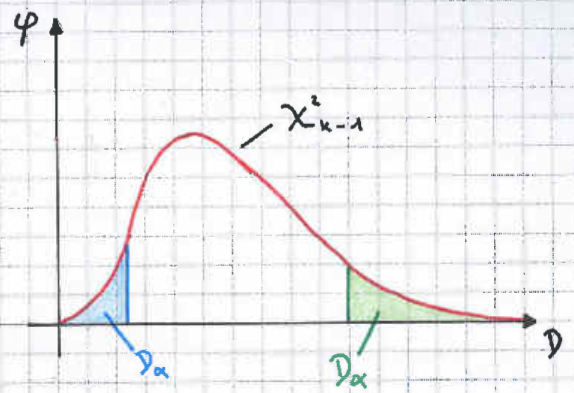
\includegraphics[width=6cm]{./bilder/chi-test.png}
        \end{minipage}\\
	\begin{tabular}{ll}
    	Nachteile:&	-Grob verpixeltes Bild der Verteilung\\
    	&			-wenn wenig Messwerte $\Longrightarrow$ geringe Aussagekraft
    \end{tabular}

\newpage
	\subsection{Kolmogorov-Smirnov Test}
	\begin{tabular}{ll}
    Idee: & Vergleiche Verteilungsfunktionen (statt der Dichtefunktionen)\\
    Daten: & $X$ Zufallsvariable, Verteilungsfunktion $F_x$, $n$ Messungen
    ergeben Stichprobe $x_i$
    \end{tabular}

	\begin{minipage}{6cm}
    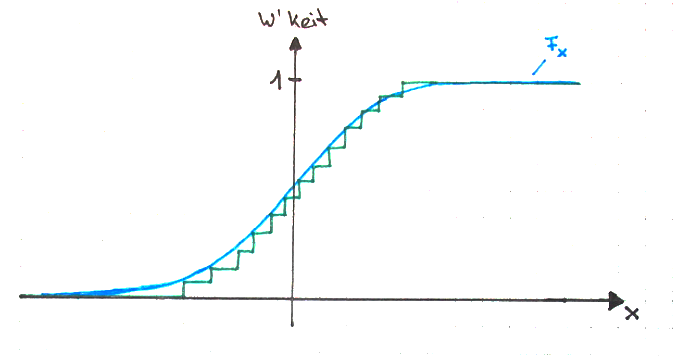
\includegraphics[width=6cm]{./bilder/ks1.png}\\
    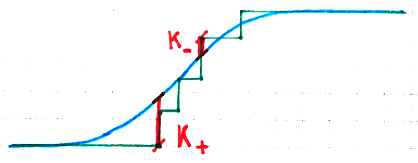
\includegraphics[width=6cm]{./bilder/ks2.png}\\
    \end{minipage}
	\begin{minipage}{12cm}
    \textcolor{blue}{$F_x$ theoretische Verteilungsfunktion}\\ \\
    \vspace{15mm}
    \textcolor{green}{empirische Verteilungsfunktion $\frac{Anzahl\{x_i \leq
    x \}}{n}$}\\

    \textcolor{red}{$K_-$ = max}
    \textcolor{blue}{$(F_x$(x)} -
    \textcolor{green}{$F_{emp}$(x))} 
    $\cdot\sqrt{n}$ \\
    \textcolor{red}{$K_{+}$ = max} 
    \textcolor{green}{$(F_{emp}(x)$}-
    \textcolor{blue}{$F_x(x))$}
    $\cdot\sqrt{n}$ \\

    \end{minipage}

	\begin{tabular}{p{18cm}}
		Sei $X1,\ldots,Xn$ sei eine Stichprobe einer Zufallsvariable $X$ . Der
		Kolmogorov- Smirnov-Test auf dem Niveau $\alpha$ für die Hypothese, 
		dass $X$ die Verteilungsfunktion $F$ hat wird wie folgt durchgeführt: \\ \\
		1. Berechne 
		$K_n^+ = \sqrt{n} \underset{-\infty<x<\infty}{max}(F(x)-F_n(x))$ und
		$K_n^- = \sqrt{n} \cdot \underset{x \in \mathbb{R}}{max}(F_n(x)-F(x))$  \\
		2. Finde $t_{n,1-\alpha}$ in der Tabelle\\ 
		3. Falls $K^+_n > t_{n,1-\alpha}$ oder $K^-_n < t_{n,\alpha}$,
		verwerfe die Hypothese, dass $X$ die Verteilungsfunktion $F$ hat. 
	\end{tabular}